\documentclass[aspectratio=169, 10pt]{beamer}

% ---------- Tema y colores ----------
\usetheme{default}
\usecolortheme{default}
\setbeamertemplate{navigation symbols}{}
\setbeamertemplate{footline}[frame number]
\setbeamertemplate{frametitle continuation}{}

\definecolor{StanfordRed}{RGB}{140,21,21}
\definecolor{StanfordGray}{RGB}{77,77,77}
\definecolor{LightGray}{RGB}{240,240,240}
\definecolor{AccentBlue}{RGB}{0,84,166}
\definecolor{AccentGreen}{RGB}{0,130,100}
\definecolor{UCMBlue}{RGB}{4, 171, 226}
\definecolor{UCMNavy}{RGB}{20, 65, 134}

% Alias de la paleta antigua: las figuras TikZ de esta clase siguen
% usando mitblue/mitgray, que ahora apuntan a los colores UCM.
\definecolor{mitblue}{RGB}{20, 65, 134}
\definecolor{mitgray}{RGB}{169, 169, 169}
\definecolor{backgroundblue}{HTML}{D7EAF3}
\definecolor{catyellow}{HTML}{FCDA76}
\definecolor{catstripe}{HTML}{F9B74C}
\definecolor{yarnred}{HTML}{E26B6B}
\definecolor{bowlblue}{HTML}{66A3D4}
\definecolor{bboxblue}{HTML}{5E69B1}
\definecolor{bboxred}{HTML}{D9534F}
\definecolor{bboxgreen}{HTML}{008000}

\setbeamercolor{frametitle}{fg=white, bg=UCMBlue}
\setbeamercolor{title}{fg=white}
\setbeamercolor{author}{fg=white}
\setbeamercolor{institute}{fg=white!80}
\setbeamercolor{structure}{fg=UCMBlue}
\setbeamercolor{block title}{bg=UCMBlue!15!white, fg=UCMBlue}
\setbeamercolor{block body}{bg=LightGray}
\setbeamercolor{block title alerted}{bg=StanfordRed!15!white, fg=StanfordRed}
\setbeamercolor{block body alerted}{bg=LightGray}
\setbeamercolor{block title example}{bg=AccentGreen!15!white, fg=AccentGreen}
\setbeamercolor{block body example}{bg=LightGray}
\setbeamercolor{alerted text}{fg=UCMBlue}
\setbeamercolor{example text}{fg=UCMBlue}

\setbeamerfont{frametitle}{series=\bfseries, size=\large}
\setbeamerfont{title}{series=\bfseries, size=\LARGE}
\setbeamerfont{block title}{series=\bfseries}

% ---------- Paquetes ----------
\usepackage[utf8]{inputenc}
\usepackage[T1]{fontenc}
\usepackage[provide=*,spanish]{babel}
\usepackage{amsmath, amssymb, bm}
\usepackage{graphicx}
\usepackage{tikz}
\usepackage{pgfplots}
\pgfplotsset{compat=1.18}
\usetikzlibrary{arrows, arrows.meta, shapes, shapes.geometric, positioning,
	fit, calc, matrix, chains, mindmap, decorations.pathreplacing,
	backgrounds, shadows, patterns}
\usepackage{booktabs}
\usepackage{xcolor}
\usepackage{multicol}
\usepackage{tcolorbox}
\tcbuselibrary{skins, breakable}
\usepackage{import}
\subimport{./layers/}{init}
\usepackage{tikzlings}


% ---------- Comandos útiles ----------
\providecommand{\R}{\mathbb{R}}
\providecommand{\E}{\mathbb{E}}
\providecommand{\Var}{\operatorname{Var}}
\providecommand{\relu}{\operatorname{ReLU}}

\newcommand{\formula}[1]{%
	\begin{tcolorbox}[colback=UCMBlue!8, colframe=UCMBlue, arc=4pt,
		boxsep=2pt, left=6pt, right=6pt, top=3pt, bottom=3pt]
		#1
	\end{tcolorbox}
}

% ---------- Portada ----------
\title{\textbf{Redes Convolucionales}}
\subtitle{Convoluci\'on, pooling y arquitecturas cl\'asicas}
\author{Sergio Hern\'andez, PhD\\ shernandez@ucm.cl}
\institute{
	\begin{tikzpicture}[scale=0.42, every node/.style={transform shape}]
		\foreach \i/\y in {1/0,2/1,3/2}{\node[circle,draw=white,fill=white!20,minimum size=4mm] (i\i) at (0,\y){};}
		\foreach \i/\y in {1/-0.5,2/0.5,3/1.5,4/2.5}{\node[circle,draw=white,fill=white!35,minimum size=4mm] (h\i) at (2,\y){};}
		\foreach \i/\y in {1/0.5,2/1.5}{\node[circle,draw=white,fill=white!50,minimum size=4mm] (o\i) at (4,\y){};}
		\foreach \a in {1,2,3}\foreach \b in {1,2,3,4}{\draw[white,opacity=0.5] (i\a)--(h\b);}
		\foreach \a in {1,2,3,4}\foreach \b in {1,2}{\draw[white,opacity=0.5] (h\a)--(o\b);}
	\end{tikzpicture}
	\\ \textbf{Mag\'ister en Data Science --- Universidad Cat\'olica del Maule}}
\date{}


\begin{document}
% --- Título ---
{
	\setbeamertemplate{background}{
		\begin{tikzpicture}[remember picture, overlay]
			\fill[UCMBlue] (current page.south west) rectangle (current page.north east);
			\fill[UCMBlue!70!black, opacity=0.5]
			(current page.south west) -- ++(0,3) -- ++(18,0) -- cycle;
			\foreach \i in {1,...,40}{
				\fill[white, opacity=0.04]
				({random()*17}, {random()*10}) circle ({random()*0.3});
			}
		\end{tikzpicture}
	}
	\begin{frame}[plain]
		\vspace{1.2cm}
		\titlepage
		\begin{tikzpicture}[remember picture, overlay]
			\node[white, opacity=0.15, font=\fontsize{80}{80}\selectfont]
			at (current page.east) [xshift=-2cm] {$\circledast$};
		\end{tikzpicture}
	\end{frame}
}

\section{Introducci\'on}
% --- Diapositiva 1: Introducción ---
% =================================================================
% SECCIÓN 1: OPTIMIZACIÓN
\begin{frame}{¿Por qué no usar solo Redes Densas (FC) para Imágenes?}
	
	\begin{block}{Explosión de Parámetros}
		Una red totalmente conectada trata una imagen como un vector plano.
		\begin{itemize}
			\item Una imagen de solo $100 \times 100$ píxeles a color (3 canales) tiene $100 \times 100 \times 3 = 30,000$ neuronas de entrada.
			\item Si la primera capa oculta tiene 1000 neuronas, ¡necesitaríamos $30,000 \times 1,000 = \textbf{30 millones}$ de pesos solo para esa capa.
			\item Esto es computacionalmente inviable y propenso al sobreajuste.
		\end{itemize}
	\end{block}

\end{frame}

\begin{frame}{¿Por qué no usar solo Redes Densas (FC) para Imágenes?}

	
	\begin{block}{Estructura Espacial}
		Al aplanar la imagen, se pierde la relación espacial entre píxeles vecinos.
		\begin{itemize}
			\item Un píxel en la esquina superior izquierda tiene la misma relación con su vecino que con un píxel en la esquina opuesta.
			\item La información visual es inherentemente \textbf{local}.
		\end{itemize}
	\end{block}
\end{frame}



% --- DIAPOSITIVA 4: PRINCIPIOS DE LAS CNNs ---
\begin{frame}{Los Principios Fundamentales de las CNNs}
	Las CNNs resuelven estos problemas basándose en dos ideas clave inspiradas en la visión humana:
	
	\begin{columns}[T]
		\begin{column}{0.5\textwidth}
			\begin{block}{1. Localidad (Locality)}
				Un píxel está fuertemente correlacionado con sus vecinos cercanos.
				\vspace{0.5cm}
				\begin{center}
					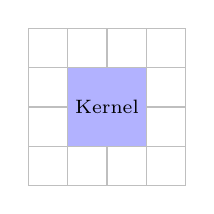
\begin{tikzpicture}
						\draw[step=0.5cm, color=gray!50] (0,0) grid (2,2);
						\fill[blue!30] (0.5,0.5) rectangle (1.5,1.5);
						\node[font=\scriptsize] at (1,1) {Kernel};
					\end{tikzpicture}
				\end{center}
				\small No necesitamos conectar cada píxel con todos los demás, solo con su vecindario local.
			\end{block}
		\end{column}
		
		\begin{column}{0.5\textwidth}
			\begin{block}{2. Invarianza a la Traslación}
				Un objeto sigue siendo el mismo objeto sin importar en qué parte de la imagen aparezca.
				\vspace{0.5cm}
				\begin{center}
					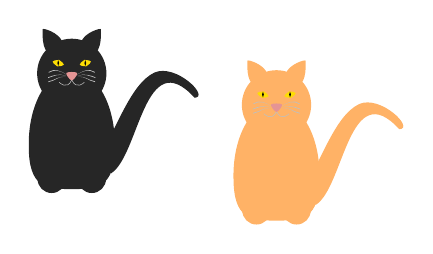
\begin{tikzpicture}
					\begin{scope}[xshift=0cm]
						\cat[xshift=0.4cm,yshift=0.4cm];
						\cat[xshift=3cm,yshift=0cm,body=orange!60];
					\end{scope}
					\end{tikzpicture}
				\end{center}
			\end{block}
		\end{column}
	\end{columns}
\end{frame}

% --- DIAPOSITIVA 5: LA OPERACIÓN DE CONVOLUCIÓN ---
\begin{frame}{Capa Convolucional}
	La convolución es una operación que extrae características locales de la imagen $g(\cdot)$ deslizando un pequeño filtro $f(\cdot)$ o \textbf{kernel} sobre ella.
	
		\begin{align}
		(f * g)(i, j) = \sum_a\sum_b f(a, b) g(i-a, j-b).
	\end{align}
	
		\begin{center}
		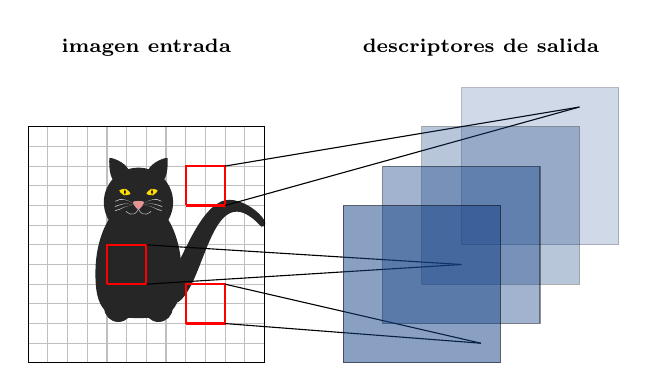
\begin{tikzpicture}
			\node[font=\scriptsize\bfseries] at (1.5,4){
				\begin{tabular}{c}
					imagen entrada
				\end{tabular}};
			\draw[step=0.25cm, color=gray!50] (0,0) grid (3,3);
			\cat[xshift=1.4cm,yshift=0.4cm];
			\draw (0,0) -- (3,0) -- (3,3) -- (0,3) -- (0,0);
			
			\draw[red,thick] (2,2) -- (2.5,2) -- (2.5,2.5) -- (2,2.5) -- (2,2);
			\draw[red,thick] (2,0.5) -- (2.5,0.5) -- (2.5,1) -- (2,1) -- (2,0.5);
			\draw[red,thick] (1,1) -- (1.5,1) -- (1.5,1.5) -- (1,1.5) -- (1,1);
			
			\draw (2.5,2) -- (7,3.25);
			\draw (2.5,2.5) -- (7,3.25);
			
			\draw (2.5,1) -- (5.75,0.25);
			\draw (2.5,0.5) -- (5.75,0.25);
			
			\draw (1.5,1.5) -- (5.5,1.25);
			\draw (1.5,1) -- (5.5,1.25);
			
			\node[font=\scriptsize\bfseries] at (5.75,4){\begin{tabular}{c}descriptores de salida\end{tabular}};
			
			\draw[fill=mitblue,opacity=0.2,draw=black] (5.5,1.5) -- (7.5,1.5) -- (7.5,3.5) -- (5.5,3.5) -- (5.5,1.5);
			\draw[fill=mitblue,opacity=0.3,draw=black] (5,1) -- (7,1) -- (7,3) -- (5,3) -- (5,1);
			\draw[fill=mitblue,opacity=0.4,draw=black] (4.5,0.5) -- (6.5,0.5) -- (6.5,2.5) -- (4.5,2.5) -- (4.5,0.5);
			\draw[fill=mitblue,opacity=0.5,draw=black] (4,0) -- (6,0) -- (6,2) -- (4,2) -- (4,0);
		\end{tikzpicture}
	\end{center}
	
\end{frame}

\begin{frame}{Convolución}
	\begin{center}
		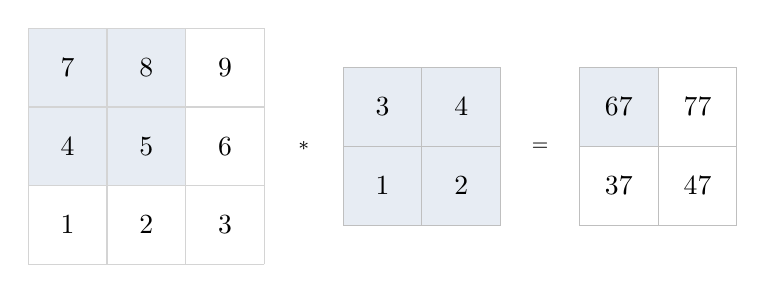
\begin{tikzpicture}				
			\draw[xshift=-4cm,step=1cm, color=mitgray!50] (0,0) grid (3,3);
			\foreach \y in {2,...,1}
			\foreach \x in {0,...,1}
				\fill[xshift=-4cm,fill=mitblue!10](\x,\y) rectangle (\x+1,\y+1) {};
			\draw[xshift=-4cm,step=1cm, color=mitgray!50] (0,0) grid (3,3);
			\foreach \y in {2,...,0}
				\foreach \x in {1,...,3}
				\pgfmathsetmacro\z{int(\x+\y*3))}
				\node[xshift=-4cm,] at (\x-0.5,\y+0.5) {\z};
				
			\node[font=\scriptsize] at (-0.5, 1.5) {$*$};
			
			\foreach \y in {1,...,0}
			\foreach \x in {1,...,2}
				\fill[xshift=-1cm,yshift=0.5cm,fill=mitblue!10](\x,\y) rectangle (\x+1,\y+1);
			
			\draw[xshift=0cm,yshift=0.5cm,step=1cm, color=gray!50] (0,0) grid (2,2);
			\foreach \y in {1,...,0}
				\foreach \x in {1,...,2}
				\pgfmathsetmacro\z{int(\x+\y*2))}
				\node[xshift=0cm,yshift=0.5cm] at (\x-0.5,\y+0.5) {\z};
				
			\node[font=\scriptsize] at (2.5, 1.5) {$=$};
			

			\fill[xshift=3cm,yshift=0.5cm,fill=mitblue!10](0,1) rectangle (1,2);
			\node[xshift=3cm,yshift=0.5cm] at (1-0.5,1+0.5) {67};
			\node[xshift=3cm,yshift=0.5cm] at (2-0.5,1+0.5) {77};
			\node[xshift=3cm,yshift=0.5cm] at (1-0.5,0.5) {37};
			\node[xshift=3cm,yshift=0.5cm] at (2-0.5,0.5) {47};
			\draw[xshift=3cm,yshift=0.5cm,step=1cm, color=gray!50] (0,0) grid (2,2);
		\end{tikzpicture}
	\end{center}
	\begin{align*}
		(7\times3)+(8\times4)+(4\times1)+(5\times2)=67,\\
		(8\times3)+(9\times4)+(5\times1)+(6\times2)=77,\\
		(4\times3)+(5\times4)+(1\times1)+(2\times2)=37,\\
		(5\times3)+(6\times4)+(2\times1)+(3\times2)=47.
	\end{align*}
\end{frame}

% --- DIAPOSITIVA 6: PADDING Y STRIDE ---
\begin{frame}{Hiperparámetros: Padding y Stride}

	
	\begin{columns}[T]
		\begin{column}{0.5\textwidth}
			\begin{block}{Padding (Relleno)}		
				\begin{itemize}
				\item Añade un borde de ceros alrededor de la imagen de entrada.
					\item Preserva las dimensiones espaciales (evitar que la imagen se encoja).
					\item Trata los píxeles de los bordes con la misma importancia que los centrales.
				\end{itemize}
				
			\end{block}
		\end{column}
		
		\begin{column}{0.5\textwidth}
		\begin{center}
			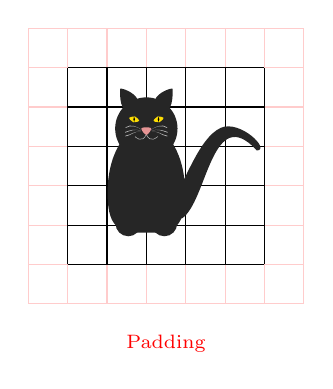
\begin{tikzpicture}[scale=1.0]
				\draw[step=0.5, red!20] (-0.5,-0.5) grid (3,3);
				\draw[step=0.5, black] (0,0) grid (2.5,2.5);
				\cat[xshift=1.0cm,yshift=0.25cm,scale=0.9];
				%\node[font=\scriptsize]  at (1.25, 1.25) {Imagen};
				%\draw[thick, red] (-0.5,-0.5) rectangle (3,3);
				\node[red,font=\scriptsize] at (1.25, -1.0) {Padding};
			\end{tikzpicture}
		\end{center}
		\end{column}
	\end{columns}
\end{frame}

\begin{frame}{Hiperparámetros: Padding y Stride}

	
	\begin{columns}[T]
		\begin{column}{0.5\textwidth}
			\begin{block}{Stride (Paso)}
			Determina el número de píxeles que el kernel se desplaza en cada paso.
		
			\begin{itemize}
				\item Un stride $> 1$ reduce drásticamente el tamaño de la salida.
				\item Permite "saltar" información y tener un campo receptivo más amplio con menos cálculos.
			\end{itemize}
			\end{block}
		\end{column}
		
		\begin{column}{0.5\textwidth}
			
				\begin{center}
					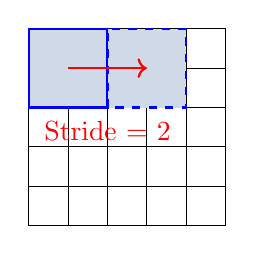
\begin{tikzpicture}[scale=1.0]
						\draw[step=0.5] (0,0) grid (2.5,2.5);
						\draw[thick, blue, fill=mitblue!20] (0,1.5) rectangle (1,2.5);
						\draw[thick, blue, fill=mitblue!20, dashed] (1,1.5) rectangle (2,2.5);
						\draw[->, thick, red] (0.5, 2) -- (1.5, 2);
						\node[red] at (1, 1.2) {Stride = 2};
					\end{tikzpicture}
				\end{center}

		\end{column}
	\end{columns}
\end{frame}

% --- DIAPOSITIVA 8: POOLING ---
\begin{frame}{Reducción de Dimensiones: La Capa de Pooling}
	Después de una capa de convolución (y una función de activación), es común aplicar una capa de Pooling.
	
	\textbf{Propósitos Principales:}
	\begin{enumerate}
		\item \textbf{Reducir las dimensiones espaciales} (alto y ancho) del mapa de características.
		\item \textbf{Reducir el costo computacional} y el número de parámetros en las capas siguientes.
		\item Hacer que la representación sea más robusta a pequeñas \textbf{traslaciones} en la entrada.
	\end{enumerate}
	
	\textbf{Tipos Comunes:}
	\begin{itemize}
		\item \textbf{Max Pooling:} Se toma el valor máximo de cada ventana. Es el más utilizado, ya que captura la característica más prominente.
		\item \textbf{Average Pooling:} Se toma el promedio de los valores de la ventana.
	\end{itemize}
\end{frame}


\begin{frame}{Sub-Muestreo (Pooling)}
	\begin{center}
		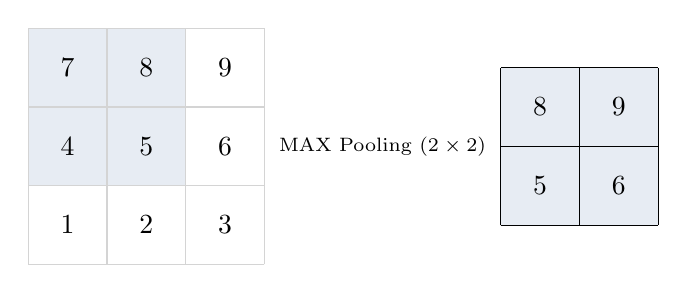
\begin{tikzpicture}				
			\draw[xshift=-4cm,step=1cm, color=mitgray!50] (0,0) grid (3,3);
			\foreach \y in {2,...,1}
			\foreach \x in {0,...,1}
			\fill[xshift=-4cm,fill=mitblue!10](\x,\y) rectangle (\x+1,\y+1) {};
			\draw[xshift=-4cm,step=1cm, color=mitgray!50] (0,0) grid (3,3);
			\foreach \y in {2,...,0}
			\foreach \x in {1,...,3}
			\pgfmathsetmacro\z{int(\x+\y*3))}
			\node[xshift=-4cm,] at (\x-0.5,\y+0.5) {\z};
			
			\node[font=\scriptsize] at (0.5, 1.5) {MAX Pooling ($2 \times 2$)};
			
			\foreach \y in {1,...,0}
			\foreach \x in {1,...,2}
			\fill[xshift=1cm,yshift=0.5cm,fill=mitblue!10](\x,\y) rectangle (\x+1,\y+1);
			
			\draw[xshift=2cm,yshift=0.5cm,step=1cm] (0,0) grid (2,2);
			\node[xshift=3cm,yshift=0.5cm] at (-0.5,1+0.5) {8};
			\node[xshift=3cm,yshift=0.5cm] at (1-0.5,1+0.5) {9};
			\node[xshift=3cm,yshift=0.5cm] at (-0.5,+0.5) {5};
			\node[xshift=3cm,yshift=0.5cm] at (1-0.5,+0.5) {6};
			
		\end{tikzpicture}
	\end{center}
	\begin{align*}
		\operatorname{MAX}(7,8,4,5)=8,\\
		\operatorname{MAX}(8,9,5,6)=9,\\
		\operatorname{MAX}(4,5,1,2)=5,\\
		\operatorname{MAX}(5,6,2,3)=6,
	\end{align*}
\end{frame}



% --- DIAPOSITIVA 7: CANALES MÚLTIPLES ---
\begin{frame}{Manejo de Múltiples Canales}
	\textbf{Imágenes a color (3 canales de entrada):}
	\begin{itemize}
		\item El kernel también debe tener 3 canales.
		\item La convolución se realiza canal por canal, y los resultados se suman para producir \textbf{un único mapa de características de salida}.
	\end{itemize}
	
\begin{center}
		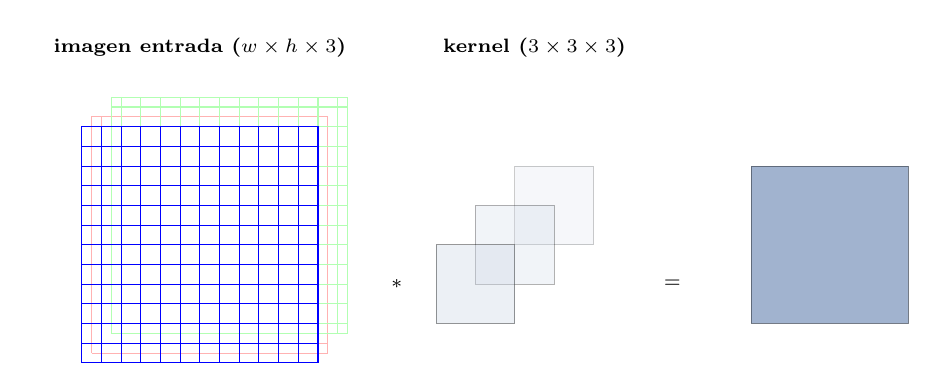
\begin{tikzpicture}
			\node[font=\scriptsize\bfseries] at (1.5,4){
				\begin{tabular}{c}
					imagen entrada ($w \times h \times 3$)
				\end{tabular}};
			\draw[step=0.25cm, color=red!30] (0.125,0.125) grid (3.125,3.125);
			\draw[red!30] (0.125,0.125) -- (3.125,0.125) -- (3.125,3.125) -- (0.125,3.125) -- (0.125,0.125);
			\draw[step=0.25cm, color=green!30] (0.375,0.375) grid (3.375,3.375);
			\draw[green!30] (0.375,0.375) -- (3.375,0.375) -- (3.375,3.375) -- (0.375,3.375) -- (0.375,0.375);
			\draw[step=0.25cm, color=blue] (0,0) grid (3,3);
			\draw[blue] (0,0) -- (3,0) -- (3,3) -- (0,3) -- (0,0);
			
			\node[font=\scriptsize\bfseries] at (4,1){$*$};
			
			\node[font=\scriptsize\bfseries] at (5.75,4){kernel ($3 \times 3 \times 3$)};
			
			\draw[fill=mitblue!20,opacity=0.2,draw=black,] (5.5,1.5) -- (6.5,1.5) -- (6.5,2.5) -- (5.5,2.5) -- (5.5,1.5);
			\draw[fill=mitblue!20,opacity=0.3,draw=black] (5,1) -- (6,1) -- (6,2) -- (5,2) -- (5,1);
			\draw[fill=mitblue!20,opacity=0.4,draw=black] (4.5,0.5) -- (5.5,0.5) -- (5.5,1.5) -- (4.5,1.5) -- (4.5,0.5);
			\node[font=\scriptsize\bfseries] at (7.5,1){$=$};
			\draw[fill=mitblue,opacity=0.4,draw=black] (8.5,0.5) -- (10.5,0.5) -- (10.5,2.5) -- (8.5,2.5) -- (8.5,0.5);
		\end{tikzpicture}
	\end{center}
		
\end{frame}

\begin{frame}
\frametitle{Red Neuronal Convolucional}
\centering
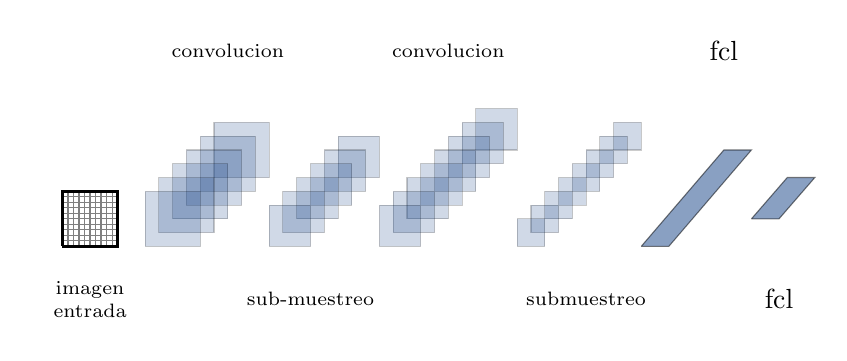
\begin{tikzpicture}[scale=.7]
	\node[font=\scriptsize] at (0.5,-1){\begin{tabular}{c}imagen\\entrada\end{tabular}};
	
	\draw[step=0.1,gray] (0,0) grid (1.0,1.0);
	\draw[very thick] (0,0) -- (1,0) -- (1,1) -- (0,1) -- (0,0);
	
	\node[font=\scriptsize] at (3,3.5){\begin{tabular}{c}convolucion\end{tabular}};
	
	\draw[fill=mitblue,opacity=0.2,draw=black] (2.75,1.25) -- (3.75,1.25) -- (3.75,2.25) -- (2.75,2.25) -- (2.75,1.25);
	\draw[fill=mitblue,opacity=0.2,draw=black] (2.5,1) -- (3.5,1) -- (3.5,2) -- (2.5,2) -- (2.5,1);
	\draw[fill=mitblue,opacity=0.2,draw=black] (2.25,0.75) -- (3.25,0.75) -- (3.25,1.75) -- (2.25,1.75) -- (2.25,0.75);
	\draw[fill=mitblue,opacity=0.2,draw=black] (2,0.5) -- (3,0.5) -- (3,1.5) -- (2,1.5) -- (2,0.5);
	\draw[fill=mitblue,opacity=0.2,draw=black] (1.75,0.25) -- (2.75,0.25) -- (2.75,1.25) -- (1.75,1.25) -- (1.75,0.25);
	\draw[fill=mitblue,opacity=0.2,draw=black] (1.5,0) -- (2.5,0) -- (2.5,1) -- (1.5,1) -- (1.5,0);
	
	\node[font=\scriptsize] at (4.5,-1){\begin{tabular}{c}sub-muestreo\end{tabular}};
	
	\draw[fill=mitblue,opacity=0.2,draw=black] (5,1.25) -- (5.75,1.25) -- (5.75,2) -- (5,2) -- (5,1.25);
	\draw[fill=mitblue,opacity=0.2,draw=black] (4.75,1) -- (5.5,1) -- (5.5,1.75) -- (4.75,1.75) -- (4.75,1);
	\draw[fill=mitblue,opacity=0.2,draw=black] (4.5,0.75) -- (5.25,0.75) -- (5.25,1.5) -- (4.5,1.5) -- (4.5,0.75);
	\draw[fill=mitblue,opacity=0.2,draw=black] (4.25,0.5) -- (5,0.5) -- (5,1.25) -- (4.25,1.25) -- (4.25,0.5);
	\draw[fill=mitblue,opacity=0.2,draw=black] (4,0.25) -- (4.75,0.25) -- (4.75,1) -- (4,1) -- (4,0.25);
	\draw[fill=mitblue,opacity=0.2,draw=black] (3.75,0) -- (4.5,0) -- (4.5,0.75) -- (3.75,0.75) -- (3.75,0);
	
	\node[font=\scriptsize] at (7,3.5){\begin{tabular}{c}convolucion\end{tabular}};
	
	\draw[fill=mitblue,opacity=0.2,draw=black] (7.5,1.75) -- (8.25,1.75) -- (8.25,2.5) -- (7.5,2.5) -- (7.5,1.75);
	\draw[fill=mitblue,opacity=0.2,draw=black] (7.25,1.5) -- (8,1.5) -- (8,2.25) -- (7.25,2.25) -- (7.25,1.5);
	\draw[fill=mitblue,opacity=0.2,draw=black] (7,1.25) -- (7.75,1.25) -- (7.75,2) -- (7,2) -- (7,1.25);
	\draw[fill=mitblue,opacity=0.2,draw=black] (6.75,1) -- (7.5,1) -- (7.5,1.75) -- (6.75,1.75) -- (6.75,1);
	\draw[fill=mitblue,opacity=0.2,draw=black] (6.5,0.75) -- (7.25,0.75) -- (7.25,1.5) -- (6.5,1.5) -- (6.5,0.75);
	\draw[fill=mitblue,opacity=0.2,draw=black] (6.25,0.5) -- (7,0.5) -- (7,1.25) -- (6.25,1.25) -- (6.25,0.5);
	\draw[fill=mitblue,opacity=0.2,draw=black] (6,0.25) -- (6.75,0.25) -- (6.75,1) -- (6,1) -- (6,0.25);
	\draw[fill=mitblue,opacity=0.2,draw=black] (5.75,0) -- (6.5,0) -- (6.5,0.75) -- (5.75,0.75) -- (5.75,0);
	
	\node[font=\scriptsize] at (9.5,-1){\begin{tabular}{c}submuestreo\end{tabular}};
	
	\draw[fill=mitblue,opacity=0.2,draw=black] (10,1.75) -- (10.5,1.75) -- (10.5,2.25) -- (10,2.25) -- (10,1.75);
	\draw[fill=mitblue,opacity=0.2,draw=black] (9.75,1.5) -- (10.25,1.5) -- (10.25,2) -- (9.75,2) -- (9.75,1.5);
	\draw[fill=mitblue,opacity=0.2,draw=black] (9.5,1.25) -- (10,1.25) -- (10,1.75) -- (9.5,1.75) -- (9.5,1.25);
	\draw[fill=mitblue,opacity=0.2,draw=black] (9.25,1) -- (9.75,1) -- (9.75,1.5) -- (9.25,1.5) -- (9.25,1);
	\draw[fill=mitblue,opacity=0.2,draw=black] (9,0.75) -- (9.5,0.75) -- (9.5,1.25) -- (9,1.25) -- (9,0.75);
	\draw[fill=mitblue,opacity=0.2,draw=black] (8.75,0.5) -- (9.25,0.5) -- (9.25,1) -- (8.75,1) -- (8.75,0.5);
	\draw[fill=mitblue,opacity=0.2,draw=black] (8.5,0.25) -- (9,0.25) -- (9,0.75) -- (8.5,0.75) -- (8.5,0.25);
	\draw[fill=mitblue,opacity=0.2,draw=black] (8.25,0) -- (8.75,0) -- (8.75,0.5) -- (8.25,0.5) -- (8.25,0);
	
	\node at (12,3.5){\begin{tabular}{c}fcl\end{tabular}};
	
	\draw[fill=mitblue,draw=black,opacity=0.5] (10.5,0) -- (11,0) -- (12.5,1.75) -- (12,1.75) -- (10.5,0);
	
	\node at (13,-1){\begin{tabular}{c}fcl\end{tabular}};
	
	\draw[fill=mitblue,draw=black,opacity=0.5] (12.5,0.5) -- (13,0.5) -- (13.65,1.25) -- (13.15,1.25) -- (12.5,0.5);
\end{tikzpicture}
fcl=fully connected layer (capa densa)
\end{frame}



% --- DIAPOSITIVA 10: ARQUITECTURA LENET-5 ---
\begin{frame}[shrink]{LeNet-5}
	LeNet-5 (Yann LeCun, 1998) es una de las primeras CNNs exitosas, diseñada para el reconocimiento de dígitos manuscritos.
	\begin{figure}
		\centering
		\resizebox{\textwidth}{!}{%
	\begin{tikzpicture}
\tikzstyle{connection}=[ultra thick,every node/.style={sloped,allow upside down},draw=gray,opacity=0.7]
\tikzstyle{copyconnection}=[ultra thick,every node/.style={sloped,allow upside down},draw={rgb:blue,4;red,1;green,1;black,3},opacity=0.7]
\pic[shift={(0,0,0)}] at (0,0,0) 
    {Box={
        name=conv0,
        caption= ,
        xlabel={{1, }},
        zlabel=32,
        fill=mitblue!50,
        height=32,
        width=1,
        depth=32
        }
    };


\pic[shift={(1,0,0)}] at (conv0-east) 
    {Box={
        name=conv1,
        caption= ,
        xlabel={{6, }},
        zlabel=28,
        fill=mitblue!50,
        height=28,
        width=6,
        depth=28
        }
    };


\draw [connection]  (conv0-east)    -- node {\midarrow} (conv1-west);


\pic[shift={ (0,0,0) }] at (conv1-east) 
    {Box={
        name=pool1,
        caption= ,
        fill=red!20,
        opacity=0.5,
        height=14,
        width=6,
        depth=14
        }
    };


\pic[shift={(1,0,0)}] at (pool1-east) 
    {Box={
        name=conv2,
        caption= ,
        xlabel={{16, }},
        zlabel=10,
        fill=mitblue!50,
        height=10,
        width=16,
        depth=10
        }
    };


\draw [connection]  (pool1-east)    -- node {\midarrow} (conv2-west);


\pic[shift={ (0,0,0) }] at (conv2-east) 
    {Box={
        name=pool2,
        caption= ,
        fill=red!20,
        opacity=0.5,
        height=5,
        width=16,
        depth=5
        }
    };


\pic[shift={(1,0,0)}] at (pool2-east) 
    {Box={
        name=conv3,
        caption= ,
        xlabel={{1, }},
        zlabel=120,
        fill=mitblue!50,
        height=1,
        width=1,
        depth=120
        }
    };


\draw [connection]  (pool2-east)    -- node {\midarrow} (conv3-west);


\pic[shift={(2,0,0)}] at (conv3-east) 
    {Box={
        name=conv4,
        caption= ,
        xlabel={{1, }},
        zlabel=84,
        fill=mitblue!50,
        height=1,
        width=1,
        depth=84
        }
    };


\draw [connection]  (conv3-east)    -- node {\midarrow} (conv4-west);


\pic[shift={(3,0,0)}] at (conv4-east) 
    {Box={
        name=soft1,
        caption=SOFT,
        xlabel={{" ","dummy"}},
        zlabel=10,
        fill=mitblue,
        opacity=0.8,
        height=3,
        width=1.5,
        depth=25
        }
    };
\draw [connection]  (conv4-east)    -- node {\midarrow} (soft1-west);
\end{tikzpicture}%
		} % Fin de resizebox
	\end{figure}

\end{frame}

\begin{frame}[shrink]{AlexNet (2012)}
	AlexNet (Krizhevsky et al., 2012) es red neuronal convolucional moderna implementada en GPU.
	\begin{figure}
		\centering
		\resizebox{\textwidth}{!}{%
	\begin{tikzpicture}
	\tikzstyle{connection}=[ultra thick,every node/.style={sloped,allow upside down},draw=gray,opacity=0.7]
\tikzstyle{copyconnection}=[ultra thick,every node/.style={sloped,allow upside down},draw={rgb:blue,4;red,1;green,1;black,3},opacity=0.7]
\pic[shift={(0,0,0)}] at (0,0,0) 
    {Box={
        name=conv0,
        caption= ,
        xlabel={{3, }},
        zlabel=224,
        fill=mitblue!50,
        height=44.8,
        width=3,
        depth=44.8
        }
    };


\pic[shift={(1,0,0)}] at (conv0-east) 
    {Box={
        name=conv1,
        caption= ,
        xlabel={{96, }},
        zlabel=55,
        fill=mitblue!50,
        height=11.0,
        width=4.8,
        depth=11.0
        }
    };


\draw [connection]  (conv0-east)    -- node {\midarrow} (conv1-west);


\pic[shift={ (0,0,0) }] at (conv1-east) 
    {Box={
        name=pool1,
        caption= ,
        fill=red!20,
        opacity=0.5,
        height=5.4,
        width=1,
        depth=5.4
        }
    };


\pic[shift={(1,0,0)}] at (pool1-east) 
    {Box={
        name=conv2,
        caption= ,
        xlabel={{256, }},
        zlabel=27,
        fill=mitblue!50,
        height=5.4,
        width=12.8,
        depth=5.4
        }
    };


\draw [connection]  (pool1-east)    -- node {\midarrow} (conv2-west);


\pic[shift={ (0,0,0) }] at (conv2-east) 
    {Box={
        name=pool2,
        caption= ,
        fill=mitblue!50,
        opacity=0.5,
        height=2.6,
        width=1,
        depth=2.6
        }
    };


\pic[shift={(1,0,0)}] at (pool2-east) 
    {Box={
        name=conv3,
        caption= ,
        xlabel={{384, }},
        zlabel=13,
        fill=mitblue!50,
        height=2.6,
        width=19.2,
        depth=2.6
        }
    };


\draw [connection]  (pool2-east)    -- node {\midarrow} (conv3-west);


\pic[shift={(1,0,0)}] at (conv3-east) 
    {Box={
        name=conv4,
        caption= ,
        xlabel={{384, }},
        zlabel=13,
        fill=mitblue!50,
        height=2.6,
        width=19.2,
        depth=2.6
        }
    };


\draw [connection]  (conv3-east)    -- node {\midarrow} (conv4-west);


\pic[shift={(1,0,0)}] at (conv4-east) 
    {Box={
        name=conv5,
        caption= ,
        xlabel={{256, }},
        zlabel=13,
        fill=mitblue!50,
        height=2.6,
        width=12.8,
        depth=2.6
        }
    };


\draw [connection]  (conv4-east)    -- node {\midarrow} (conv5-west);


\pic[shift={ (0,0,0) }] at (conv5-east) 
    {Box={
        name=pool3,
        caption= ,
        fill=red!20,
        opacity=0.5,
        height=1.2,
        width=1,
        depth=1.2
        }
    };


\pic[shift={(1,0,0)}] at (pool3-east) 
    {Box={
        name=Fc1,
        caption= ,
        xlabel={{1, }},
        zlabel=4096,
        fill=mitblue,
        height=1,
        width=1,
        depth=40.96
        }
    };


\draw [connection]  (pool3-east)    -- node {\midarrow} (Fc1-west);


\pic[shift={(2,0,0)}] at (Fc1-east) 
    {Box={
        name=Fc2,
        caption= ,
        xlabel={{1, }},
        zlabel=4096,
        fill=mitblue,
        height=1,
        width=1,
        depth=40.96
        }
    };


\draw [connection]  (Fc1-east)    -- node {\midarrow} (Fc2-west);


\pic[shift={(3,0,0)}] at (Fc2-east) 
    {Box={
        name=soft1,
        caption=SOFTMAX,
        xlabel={{" ","dummy"}},
        zlabel=1000,
        fill=mitblue,
        opacity=0.8,
        height=3,
        width=1.5,
        depth=25
        }
    };


\draw [connection]  (Fc2-east)    -- node {\midarrow} (soft1-west);
\end{tikzpicture}%
		} % Fin de resizebox
	\end{figure}

\end{frame}

\begin{frame}{VGG16 (2014)}
	En VGG16 (Simonyan y Zisserman, 2014) los autores usan múltiples convoluciones y sub-sampleo para construir bloques que pueden ser apilados en capas sucesivas.
	\begin{figure}
		\centering
		\resizebox{\textwidth}{!}{%
	\begin{tikzpicture}
	\tikzstyle{connection}=[ultra thick,every node/.style={sloped,allow upside down},draw=gray,opacity=0.7]
\tikzstyle{copyconnection}=[ultra thick,every node/.style={sloped,allow upside down},draw={rgb:blue,4;red,1;green,1;black,3},opacity=0.7]
\pic[shift={(0,0,0)}] at (0,0,0) {RightBandedBox={name=cr1,caption=conv1,%
        xlabel={{"64","64"}},ylabel=224,zlabel=224,fill=mitblue!50,bandfill=mitblue!50,%
        height=40,width={2,2},depth=40}};
%pool1
\pic[shift={(0,0,0)}] at (cr1-east) {Box={name=p1,%
        fill=red!20,opacity=0.5,height=35,width=1,depth=35}};
%%%%%%%%%%
% conv2_1,conv2_2
\pic[shift={(2,0,0)}] at (p1-east) {RightBandedBox={name=cr2,caption=conv2,%
        xlabel={{"128","128"}},zlabel=112,fill=mitblue!50,bandfill=mitblue!50,%
        height=35,width={3,3},depth=35}};
%pool2
\pic[shift={(0,0,0)}] at (cr2-east) {Box={name=p2,%
        fill=red!20,opacity=0.5,height=30,width=1,depth=30}};
%%%%%%%%%%
% conv3_1,conv3_2
\pic[shift={(2,0,0)}] at (p2-east) {RightBandedBox={name=cr3,caption=conv3,%
        xlabel={{"256","256","256"}},zlabel=56,fill=mitblue!50,bandfill=mitblue!50,%
        height=30,width={4,4,4},depth=30}};
%pool3
\pic[shift={(0,0,0)}] at (cr3-east) {Box={name=p3,%
        fill=red!20,opacity=0.5,height=23,width=1,depth=23}};
%%%%%%%%%%
% conv4_1,conv4_2,conv4_3
\pic[shift={(1.8,0,0)}] at (p3-east) {RightBandedBox={name=cr4,caption=conv4,%
        xlabel={{"512","512","512"}},zlabel=28,fill=mitblue!50,bandfill=mitblue!50,%
        height=23,width={7,7,7},depth=23}};
%pool4
\pic[shift={(0,0,0)}] at (cr4-east) {Box={name=p4,%
        fill=red!20,opacity=0.5,height=15,width=1,depth=15}};
%%%%%%%%%%
% conv5_1,conv5_2,conv5_3
\pic[shift={(1.5,0,0)}] at (p4-east) {RightBandedBox={name=cr5,caption=conv5,%
        xlabel={{"512","512","512"}},zlabel=14,fill=mitblue!50,bandfill=mitblue!50,%
        height=15,width={7,7,7},depth=15}};
%pool5
\pic[shift={(0,0,0)}] at (cr5-east) {Box={name=p5,%
        fill=red!20,opacity=0.5,height=10,width=1,depth=10}};
%%%%%%%%%%
% fc6
\pic[shift={(3,0,0)}] at (p5-east) {RightBandedBox={name=fc6,caption=fc6,%
        xlabel={{"1",""}},zlabel=4096,fill=mitblue,bandfill=mitblue!50,%
        height=3,width=3,depth=100}};
%%%%%%%%%%
% fc7
\pic[shift={(2,0,0)}] at (fc6-east) {RightBandedBox={name=fc7,caption=fc7,%
        xlabel={{"1","dummy"}},zlabel=4096,fill=mitblue,bandfill=mitblue!50,%
        height=3,width=3,depth=100}};
%%%%%%%%%%
% fc8
\pic[shift={(1.5,0,0)}] at (fc7-east) {RightBandedBox={name=fc8,caption=fc8+softmax,%
        xlabel={{"1","dummy"}},fill=mitblue,bandfill=mitblue!50,%
        height=3,width=3,depth=25}};

%%%%%%%%%%
% softmax
\pic[shift={(0,0,0)}] at (fc8-east) {Box={name=softmax,%
        xlabel={{"","dummy"}},zlabel=K,opacity=0.8,fill=mitblue,%
        height=3,width=1.5,depth=25}};
    
%%%%%%%%%%%%%%%%%%%%%%%%%%%%%%%%%%%%%%%%%%%%%%%%%%%%%%%%%%%%%%%%%%%%%%%%%%%%%%%%%%%%%%%%
%% Draw Arrow Connections
%%%%%%%%%%%%%%%%%%%%%%%%%%%%%%%%%%%%%%%%%%%%%%%%%%%%%%%%%%%%%%%%%%%%%%%%%%%%%%%%%%%%%%%%
\draw [connection]  (p1-east)        -- node {\midarrow} (cr2-west);
\draw [connection]  (p2-east)        -- node {\midarrow} (cr3-west);
\draw [connection]  (p3-east)        -- node {\midarrow} (cr4-west);
\draw [connection]  (p4-east)        -- node {\midarrow} (cr5-west);
\draw [connection]  (p5-east)        -- node {\midarrow} (fc6-west);
\draw [connection]  (fc6-east)       -- node {\midarrow} (fc7-west);
\draw [connection]  (fc7-east)       -- node {\midarrow} (fc8-west);
\draw [connection]  (softmax-east)   -- node {\midarrow} ++(1.5,0,0);
%%%%%%%%%%%%%%%%%%%%%%%%%%%%%%%%%%%%%%%%%%%%%%%%%%%%%%%%%%%%%%%%%%%%%%%%%%%%%%%%%%%%%%%%
%% Draw Dotted Edges 
%%%%%%%%%%%%%%%%%%%%%%%%%%%%%%%%%%%%%%%%%%%%%%%%%%%%%%%%%%%%%%%%%%%%%%%%%%%%%%%%%%%%%%%%
\draw[densely dashed]
    (fc6-west)++(0, 1.5*.2, 1.5*.2) coordinate(a) -- (p5-nearnortheast)
    (fc6-west)++(0,-1.5*.2, 1.5*.2) coordinate(b) -- (p5-nearsoutheast)
    (fc6-west)++(0,-1.5*.2,-1.5*.2) coordinate(c) -- (p5-farsoutheast)
    (fc6-west)++(0, 1.5*.2,-1.5*.2) coordinate(d) -- (p5-farnortheast)
    
    (a)--(b)--(c)--(d)
    ;
%%%%%%%%%%%%%%%%%%%%%%%%%%%%%%%%%%%%%%%%%%%%%%%%%%%%%%%%%%%%%%%%%%%%%%%%%%%%%%%%%%%%%%%%
\end{tikzpicture}%
		} % Fin de resizebox
	\end{figure}

\end{frame}

\begin{frame}[shrink]{ResNet (2016)}
	En ResNet (He et.al, 2016) los autores proponen normalización de lotes (BatchNorm) y bloques residuales (cortocircuito) del tipo $g(x)=f(x)-x$.
	\begin{figure}
		\centering
		\resizebox{\textwidth}{!}{%
			\begin{tikzpicture}
				\tikzstyle{connection}=[ultra thick,every node/.style={sloped,allow upside down},draw=\edgecolor,opacity=0.7]
				\tikzstyle{copyconnection}=[ultra thick,every node/.style={sloped,allow upside down},draw={rgb:blue,4;red,1;green,1;black,3},opacity=0.7]
				
				%%%%%%%%%%%%%%%%%%%%%%%%%%%%%%%%%%%%%%%%%%%%%%%%%%%%%%%%%%%%%%%%%%%%%%%%%%%%%%%%%%%%%%%%
				%% Draw Encoder
				%%%%%%%%%%%%%%%%%%%%%%%%%%%%%%%%%%%%%%%%%%%%%%%%%%%%%%%%%%%%%%%%%%%%%%%%%%%%%%%%%%%%%%%%
				
				\path (-4,0,0);
				% input
				\pic[shift={(0,0,0)}] at (0,0,0) {
					Box={
						name=input,
						caption=Input,
						xlabel= 3,
						ylabel=224,
						zlabel= \qquad 224,
						fill=mitblue!20,
						height=100,
						width=0.1,
						depth=100
					}
				};
				% conv1
				\pic[shift={(1.5,0,0)}] at (input-east) {
					RightBandedBox={
						name= conv1,
						caption=Conv1,
						xlabel={{"64",""}},
						ylabel=112,
						zlabel= \qquad 112,
						fill=mitblue!20,
						bandfill=mitblue!20,
						height=50,
						width=2.1,
						depth=50
					}
				};
				% MaxPool2d
				\pic[shift={(1,0,0)}] at (conv1-east) {
					RightBandedBox={
						name= MaxPool,
						xlabel={{"64",""}},
						ylabel=112,
						fill=red!20,
						height=50,
						width=2.1,
						depth=50
					}
				};
				
				
				
				% layer1
				% conv1_1
				\pic[shift={(3,0,0)}] at (MaxPool-east) {
					RightBandedBox={
						name= conv1_1,
						xlabel={{"64",""}},
						ylabel= 112,
						fill=mitblue!20,
						bandfill=mitblue!20,
						height=50,
						width=2.1,
						depth=50
					}
				};
				% conv1_2
				\pic[shift={(0,0,0)}] at (conv1_1-east) {
					RightBandedBox={
						name= conv1_2,
						xlabel={{"\quad 64",""}},
						zlabel= \qquad 112,
						fill=mitblue!20,
						bandfill=mitblue!20,
						height=50,
						width=2.1,
						depth=50
					}
				};
				% add1_1
				\pic[shift={(1,0,0)}] at (conv1_2-east) {
					Ball={
						name=add1_1,
						fill=red!20,
						opacity=0.6,
						radius=2,
						logo=\(+\)
					}
				};
				\pic[shift={(-0.2,0,0)}] at (conv1_1-west) {Box={name=env,caption=\textbf{\large{$\times$ 3}},%
						xlabel={{"","dummy"}},fill=,opacity=0.1,height=60,width={10},depth=60}};
				
				%%%%%%%%%%%%%%%%%%%%%%%%%%%%%%%%%%
				\pic[shift={(3,0,0)}] at (conv1_2-east) {
					RightBandedBox={
						name= conv2_1,
						xlabel={{"128",""}},
						ylabel= 56,
						fill=mitblue!20,
						bandfill=mitblue!20,
						height=25,
						width=4.2,
						depth=25
					}
				};
				% conv2_2
				\pic[shift={(0,0,0)}] at (conv2_1-east) {
					RightBandedBox={
						name= conv2_2,
						xlabel={{"128",""}},
						zlabel= \qquad 56,
						fill=mitblue!20,
						bandfill=mitblue!20,
						height=25,
						width=4.2,
						depth=25
					}
				};
				
				% add1_2
				\pic[shift={(1,0,0)}] at (conv2_2-east) {
					Ball={
						name=add1_2,
						fill=red!20,
						opacity=0.6,
						radius=2,
						logo=\(+\)
					}
				};
				\pic[shift={(-0.4,0,0)}] at (conv2_1-west) {Box={name=env,caption=\textbf{\large{$\times$ 4}},%
						xlabel={{"","dummy"}},fill=,opacity=0.1,height=30,width={20},depth=30}};
				
				%%%%%%%%%%%%%%%%%%%%%%%%%%%%%%%%%%%%%%%%%%%%%%%%%
				% conv3_1
				\pic[shift={(3,0,0)}] at (conv2_2-east) {
					RightBandedBox={
						name= conv3_1,
						xlabel={{"256",""}},
						ylabel= 28,
						fill=mitblue!20,
						bandfill=mitblue!20,
						height=12.5,
						width=8.4,
						depth=12.5
					}
				};
				% conv3_2
				\pic[shift={(0,0,0)}] at (conv3_1-east) {
					RightBandedBox={
						name= conv3_2,
						xlabel={{"256",""}},
						zlabel= 28,
						fill=mitblue!20,
						bandfill=mitblue!20,
						height=12.5,
						width=8.4,
						depth=12.5
					}
				};
				
				% add1_3
				\pic[shift={(1,0,0)}] at (conv3_2-east) {
					Ball={
						name=add1_3,
						fill=red!20,
						opacity=0.6,
						radius=2,
						logo=\(+\)
					}
				};
				\pic[shift={(-0.6,0,0)}] at (conv3_1-west) {Box={name=env,caption=\textbf{\large{$\times$ 6}},%
						xlabel={{"","dummy"}},fill=,opacity=0.1,height=20,width={30},depth=20}};
				%%%%%%%%%%%%%%%%%%%%%%%%%%%%%%%%%%%%%%%%%
				
				% conv4_1
				\pic[shift={(3,0,0)}] at (conv3_2-east) {
					RightBandedBox={
						name= conv4_1,
						xlabel={{"512",""}},
						ylabel= 14,
						fill=mitblue!20,
						bandfill=mitblue!20,
						height=6.25,
						width=16.8,
						depth=6.25
					}
				};
				% conv4_2
				\pic[shift={(0,0,0)}] at (conv4_1-east) {
					RightBandedBox={
						name= conv4_2,
						xlabel={{"512",""}},
						ylabel= 14,
						fill=mitblue!20,
						bandfill=mitblue!20,
						height=6.25,
						width=16.8,
						depth=6.25
					}
				};
				
				% add1_4
				\pic[shift={(1,0,0)}] at (conv4_2-east) {
					Ball={
						name=add1_4,
						fill=red!20,
						opacity=0.6,
						radius=2,
						logo= \(+\)
					}
				};
				\pic[shift={(-0.8,0,0)}] at (conv4_1-west) {Box={name=env,caption=\textbf{\large{$\times$ 3}},%
						xlabel={{"","dummy"}},fill=,opacity=0.1,height=15,width={48},depth=15}};
				
				% avgpool
				\pic[shift={(3,0,0)}] at (add1_4-east) {
					Box={
						name=avgpool,
						caption= \\ avgpool,
						xlabel={{"1",""}},
						ylabel=1,
						zlabel=\qquad 512,
						fill=red!20,
						height=2,
						width=2,
						depth=150
					}
				};
				
				
				% fullconnection
				\pic[shift={(2,0,0)}] at (avgpool-east) {
					RightBandedBox={
						name=fc,
						caption=\makebox[0pt]{
							\shortstack[c]{\\ full \, connection\\softmax}},
						xlabel={{"1",""}},
						zlabel=\qquad 7,
						fill=mitblue!50,
						bandfill=mitblue!50,
						height=2,
						width=2,
						depth=20
					}
				};
				
				% connections
				\draw [connection]  		(input-east)			-- 	node {\midarrow} 	(conv1-west);
				\draw [connection]  		(conv1-east)			-- 	node {\midarrow} 	(MaxPool-west);
				\draw [connection] (MaxPool-east) -- node {\midarrow} (conv1_1-west);
				
				
				% connections shortcut
				% conv1 to add1_1
				\path (MaxPool-east) -- (conv1_1-west) coordinate[pos=0.5] (pool_conv1_1);
				\path (pool_conv1_1) ++ (0,5,0) coordinate (pool_conv1_1_above);
				\path (add1_1-north) ++ (0,5,0) coordinate (add1_1-north-above);
				
				\draw [connection] (pool_conv1_1) -- node {\midarrow} (pool_conv1_1_above|-add1_1-north-above) -- node {\midarrow} (add1_1-north-above) -- node {\midarrow} (add1_1-north);
				\draw [connection] (conv1_2-east) -- (add1_1-west);
				\draw [connection] (add1_1-east) -- node {\midarrow} (conv2_1-west);
				
				%
				\path (conv1_2-east) -- (conv2_1-west) coordinate[pos=0.65] (add_conv_1);
				\path (add_conv_1) ++ (0,5,0) coordinate (add_conv_1-above);
				\path (add1_2-north) ++ (0,5,0) coordinate (add1_2-north-above);
				\draw [connection] (add_conv_1) -- node {\midarrow} (add_conv_1-above|-add1_2-north-above) -- node {\midarrow} (add1_2-north-above) -- node {\midarrow} (add1_2-north);
				\draw [connection] (conv2_2-east) -- (add1_2-west);
				\draw [connection] (add1_2-east) -- node {\midarrow} (conv3_1-west);
				%%%%%%%%%%%%%%
				\path (conv2_2-east) -- (conv3_1-west) coordinate[pos=0.75] (add_conv_2);
				\path (add_conv_2) ++ (0,5,0) coordinate (add_conv_2-above);
				\path (add1_3-north) ++ (0,5,0) coordinate (add1_3-north-above);
				\draw [connection] (add_conv_2) -- node {\midarrow} (add_conv_2-above|-add1_3-north-above) -- node {\midarrow} (add1_3-north-above) -- node {\midarrow} (add1_3-north);
				\draw [connection] (conv3_2-east) -- (add1_3-west);
				\draw [connection] (add1_3-east) -- node {\midarrow} (conv4_1-west);
				%%%%%%%%%%%%%%%
				\path (conv3_2-east) -- (conv4_1-west) coordinate[pos=0.75] (add_conv_3);
				\path (add_conv_3) ++ (0,5,0) coordinate (add_conv_3-above);
				\path (add1_4-north) ++ (0,5,0) coordinate (add1_4-north-above);
				\draw [connection] (add_conv_3) -- node {\midarrow} (add_conv_3-above|-add1_4-north-above) -- node {\midarrow} (add1_4-north-above) -- node {\midarrow} (add1_4-north);
				\draw [connection] (conv4_2-east) -- (add1_4-west);
				%\draw [connection] (add1_4-east) -- node {\midarrow} (conv4_1-west);
				\draw [connection](add1_4-east) -- node {\midarrow}(avgpool-west);
				\draw [connection](avgpool-east) -- node {\midarrow}(fc-west);
				% pool & fullconnection
				\draw	[densely dashed]  (avgpool-nearnortheast)    	--  									(fc-nearnorthwest);
				\draw	[densely dashed]  (avgpool-nearsoutheast)    	--  									(fc-nearsouthwest);
				\draw	[densely dashed]  (avgpool-farnortheast)    	--  									(fc-farnorthwest);
				\draw	[densely dashed]  (avgpool-farsoutheast)    	--  									(fc-farsouthwest);
				%
				%%%%%%%%%%%%%%%%%%%%%%%%%%%%%%%%%%%%%%%%%%%%%%%%%%%%%%%%%%%%%%%%%%%%%%%%%%%%%%%%%%%%%%%
			\end{tikzpicture}%
		} % Fin de resizebox
	\end{figure}
	
\end{frame}

% --- DIAPOSITIVA 11: RESUMEN ---
\begin{frame}{Conclusiones}
	\begin{itemize}
		\item Las CNNs son el estándar para tareas de visión por computadora porque respetan la \textbf{estructura espacial} de las imágenes.
		\item Sus bloques de construcción principales son:
		\begin{itemize}
			\item \textbf{Capas Convolucionales:} Usan kernels (filtros) para aprender y detectar características locales.
			\item \textbf{Capas de Pooling:} Reducen las dimensiones para hacer el modelo más eficiente y robusto.
		\end{itemize}
		\item La arquitectura típica alterna estas capas de extracción de características y finaliza con capas densas para realizar la clasificación o regresión.
		\item Las CNNs no solo son potentes, sino también mucho más eficientes en parámetros que las redes densas gracias al \textbf{uso compartido de pesos}.
	\end{itemize}
\end{frame}



\end{document}